\documentclass[tikz,border=2pt]{standalone}
\usepackage{tikz}
\usetikzlibrary{shapes.geometric,arrows.meta,chains,positioning,quotes}
\begin{document}
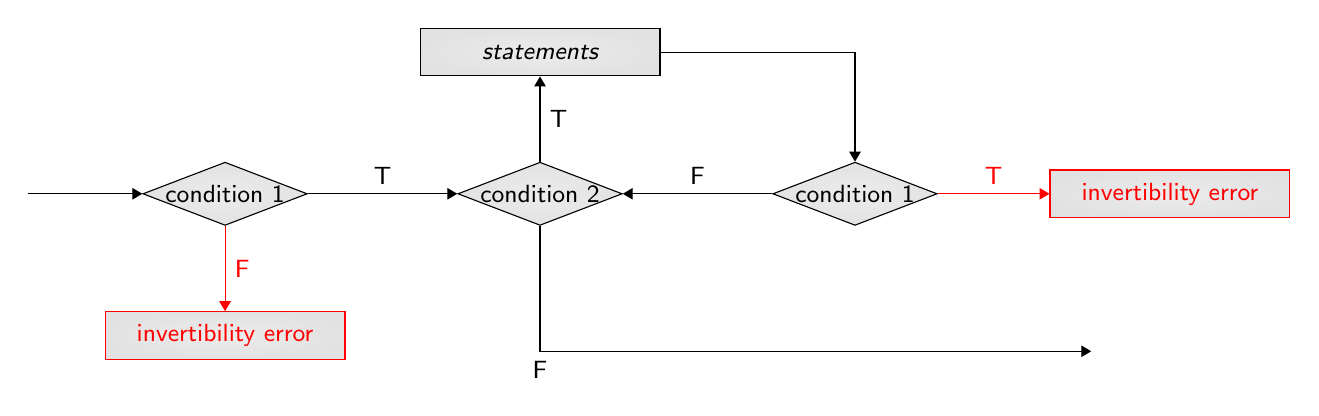
\begin{tikzpicture}[    font=\sffamily\small,
    >={Triangle[]},
    */.tip={Circle[]},
    start chain=going below,
    node distance=18mm and 40mm,
    every join/.style={norm},
    base/.style={draw, on chain, on grid, align=center, minimum height=4ex, inner color=black!50!gray!10, outer color=black!50!gray!15},
    proc/.style={base, rectangle, text width=8em},
    test/.style={base, diamond, text centered, aspect=2.6,inner sep=-0ex},
    norm/.style={->, draw, black},
    it/.style={font={\sffamily\small\itshape}}]

\node [test] (c1) {condition 1};
\node [test] (c2) [right=of c1]  {condition 2};
\node [test] (c3) [right=of c2]  {condition 1};
\node [proc, it] (st1) [above=of c2] {statements};
\node [proc,red] (err1) [below=of c1] {invertibility error};
\node [proc,red] (err2) [right=of c3] {invertibility error};
\draw [->,black] (c2) -- (st1) node[midway,right] {T};
\draw [->,black] (st1) -| (c3);
\draw [->,black] (-2.5, 0.0) -- (c1.west);
\draw [->,black] (c1) -- (c2) node[midway,above] {T};
\draw [->,black] (c3) -- (c2) node[midway,above] {F};
\draw [->,red] (c1) -- (err1) node[midway,right] {F};
\draw [->,red] (c3) -- (err2) node[midway,above] {T};
\draw [->,black] (c2.south) |- (11, -2) node[midway,below] {F};

\end{tikzpicture}
\end{document}
